\documentclass[svgnames,11pt]{beamer}
\input{/home/tof/Documents/Cozy/latex-include/preambule_commun.tex}
\input{/home/tof/Documents/Cozy/latex-include/preambule_beamer.tex}
%\usepackage{pgfpages} \setbeameroption{show notes on second screen=left}
\author[]{Christophe Viroulaud}
\title{Exercices type bac\\SoC - routage}
\date{\framebox{\textbf{Archi 19}}}
%\logo{}
\institute{Terminale - NSI}

\begin{document}
\begin{frame}
\titlepage
\end{frame}
\begin{frame}
    \frametitle{}

    Avantages SoC:
    \begin{itemize}
        \item coût de production 
        \item taille réduite
        \item moindre consommation électrique (notamment grâce à la faible longueur des BUS)
    \end{itemize}

\end{frame}
\begin{frame}
    \frametitle{}

    Situation d'interblocage:
    \begin{itemize}
        \item rétention et attente: plusieurs applications possèdent une donnée et en attendent une autre.
        \item attente circulaire 
    \end{itemize}
    On peut également évoquer la non préemption ici même si ce n'est pas dit explicitement. Il suffit qu'une des conditions de Coffman soit applicable pour risquer une situation d'interblocage.

\end{frame}
\begin{frame}
    \frametitle{}
D'après la table de routage de A, il faut passer par le routeur B pour rejoindre F. On poursuit ensuite la lecture dans la table de B\dots
    \begin{center}
        A - B - E - F
    \end{center}

\end{frame}
\begin{frame}
    \frametitle{}
Les liens \emph{directs} sont ceux dont la passerelle est identique à la destination.
    \begin{center}
        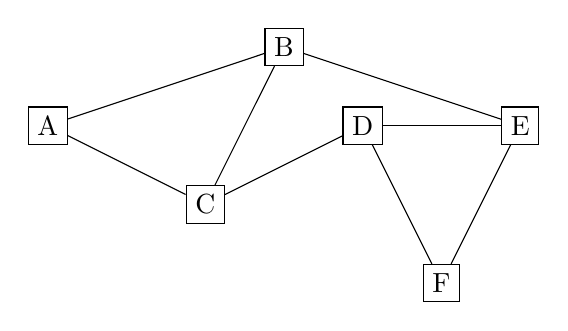
\begin{tikzpicture}
            \node[draw] (A) at(0,0){A};
            \node[draw] (B) at(3,1){B};
            \node[draw] (C) at(2,-1){C};
            \node[draw] (D) at(4,0){D};
            \node[draw] (E) at(6,0){E};
            \node[draw] (F) at(5,-2){F};

            \draw (A)--(B);
            \draw (A)--(C);
            \draw (C)--(B);
            \draw (C)--(D);
            \draw (E)--(F);
            \draw (F)--(D);
            \draw (E)--(D);
            \draw (E)--(B);

        \end{tikzpicture}
    \end{center}

\end{frame}
\end{document}